\begin{sidewaysfigure}
  \centering
  \begin{minipage}{.7\textwidth} % adjust the width as needed

    \begin{minipage}{\textwidth}
      \centering
      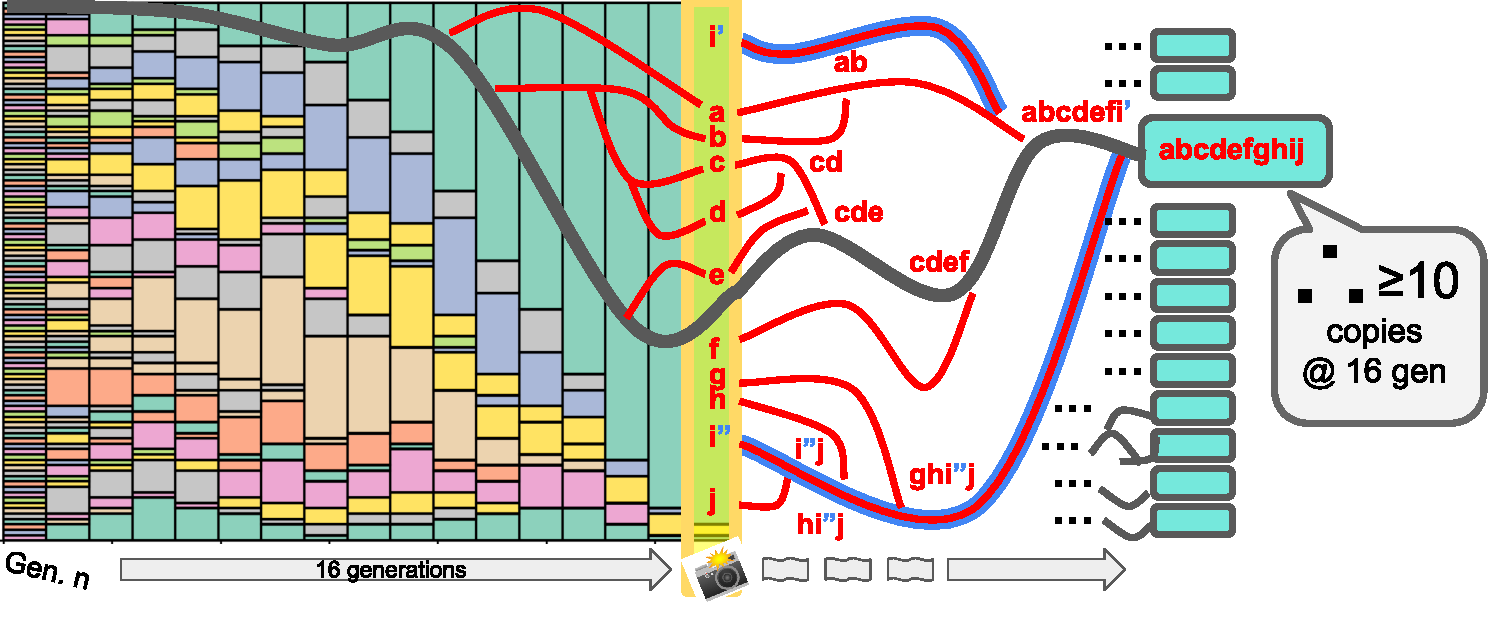
\includegraphics[height=0.30\textheight]{img/copy-count-snapshot}
      \subcaption{Cartoon depiction of delayed copy count estimation mechanism, annotated over Muller plot depicting weak selection over focal allele.
      }
      % \label{fig:ne-example-replicates:bottleneck}
    \end{minipage}%

    \vspace{1cm}

    \begin{minipage}{0.47\textwidth}
      \centering
      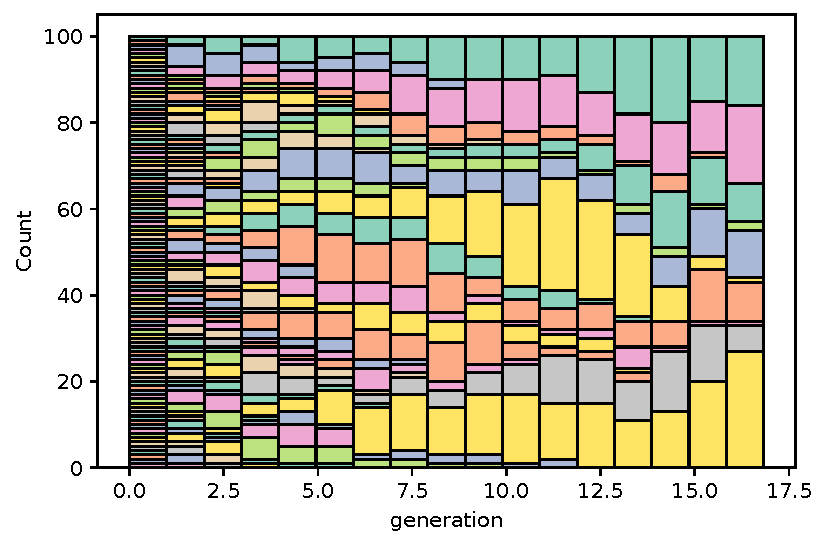
\includegraphics[height=0.2\textheight]{notebooks/notebooks/teeplots/fit=0.0+hue=clade+multiple=stack+ngen=16+npop=100+palette=set2+viz=histplot+x=generation+ext=}
      \subcaption{Muller plot depicting no selection for focal allele, ending with smaller copy count after 16 generations.}
      % \label{fig:ne-example-replicates:selection_pressure}
    \end{minipage}
    \,
    \begin{minipage}{0.47\textwidth}
      \centering
      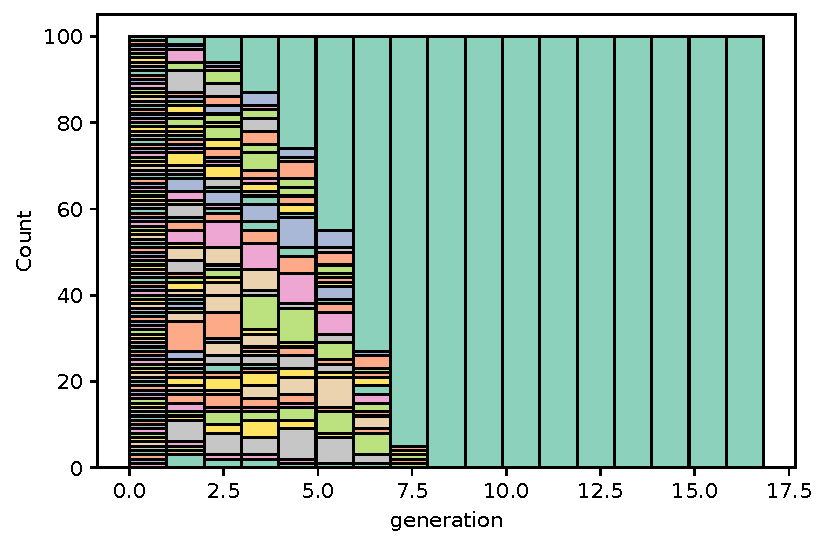
\includegraphics[height=0.2\textheight]{notebooks/notebooks/teeplots/fit=1.0+hue=clade+multiple=stack+ngen=16+npop=100+palette=set2+viz=histplot+x=generation+ext=}
      \subcaption{Muller plot depicting strong selection for focal allele, with fixation occuring before 16 generations.}
      % \label{fig:ne-example-replicates:control}
    \end{minipage}

  \end{minipage}
  \hfill % Creates horizontal space. Can also use \hspace{<len>}
  \begin{minipage}{.25\textwidth} % adjust the width as needed
    \caption{
      Proposed mechanism for detecting gene-level selection via a distributed delayed copy count estimation mechanism.
      Strata deposited at generation $n$ progress through 16 generations, with copy count of one allele growing due to selection.
      On the sixteenth generation, a ``snapshot'' is performed to set a random bit of the field annotated onto each descendant differentia copy (here, denoted by letter).
      In subsequent recombination events, set bits are exchanged between bit fields associated with common differentia.
      Copy count at generation $n + 16$ from can then be estimated from these bit fields, with high copy count indicative of selection.
      Note that in this example collision between set bits $i'$ and $i"$ result in an undercount.
      This mechanism is associated with ``gene-level'' instrumentation (Figure \ref{fig:annotation-types}).
    }
    \label{fig:ne-example-replicates}
  \end{minipage}

\end{sidewaysfigure}


% notebooks/notebooks/teeplots/notebook=ne-inference+replicate=0+treatment=bottleneck+viz=plot-running-estimation+x=rank+y=population-size+ext=.pdf
%
% notebooks/notebooks/teeplots/notebook=ne-inference+replicate=0+treatment=control+viz=plot-running-estimation+x=rank+y=population-size+ext=.pdf
%
% notebooks/notebooks/teeplots/notebook=ne-inference+replicate=0+treatment=range-expansion+viz=plot-running-estimation+x=rank+y=population-size+ext=.pdf
%
% notebooks/notebooks/teeplots/notebook=ne-inference+replicate=0+treatment=selection-pressure+viz=plot-running-estimation+x=rank+y=population-size+ext=.pdf
